\chapter{Community communication} \label{community}

\paragraph{[Wikitech-ambassadors] Looking for small Wikipedias to test a new feature for them} ~\\
\begin{quote}
As part of my Bachelor’s thesis I worked on an extension called “ArticlePlaceholder” \url{https://www.mediawiki.org/wiki/Extension:ArticlePlaceholder} over the last months. \\
\\
One of the biggest barriers for accessing the knowledge Wikipedia provides is language. \\
\\
There are many topics that are only covered in few, big Wikipedias. People who don’t speak any of these languages don’t have access to all the information available potentially vital to them. \\
\\
The Article Placeholder extensions aims at smaller Wikipedias to support them in increasing access to data available on Wikidata. Article Placeholders are automatically generated content pages in Wikipedia or other mediawiki projects displaying data from Wikidata. They are clearly not actual articles but an overview of data on a topic which does not have an article yet. The design of the page and its content is under the control of the local community via Lua and templates but we will provide defaults so smaller Wikipedias can work with them without having to worry about the technical side of it. \\
\\
I have a test setup on Labs with an example for Ada Lovelace \url{http://articleplaceholder.wmflabs.org/mediawiki/index.php/Special:AboutTopic/Q3} \\
\\
The reader can find these pages by searching for a topic and gets results if there is an Item on Wikidata with the respective label and/or alias. \\
\\
The reader would benefit a lot since even if there is no article on a topic yet, they will still have basic information provided in their language. But it also might increase the numbers of editors due to increased usefulness of that Wikipedia. \\
\\
We are now looking for the first Wikipedias to support the extension by deploying it and giving their input. I am still developing the extension and the first Wikipedias to try it will naturally have a larger say in how it evolves. \\
\\
If your Wikipedia would like to give it a try please let me know. We would start it as a beta feature. \\
\\
Thank you, \\
\\
Lucie (Frimelle)
\end{quote}
\citep{kaffee:01} 

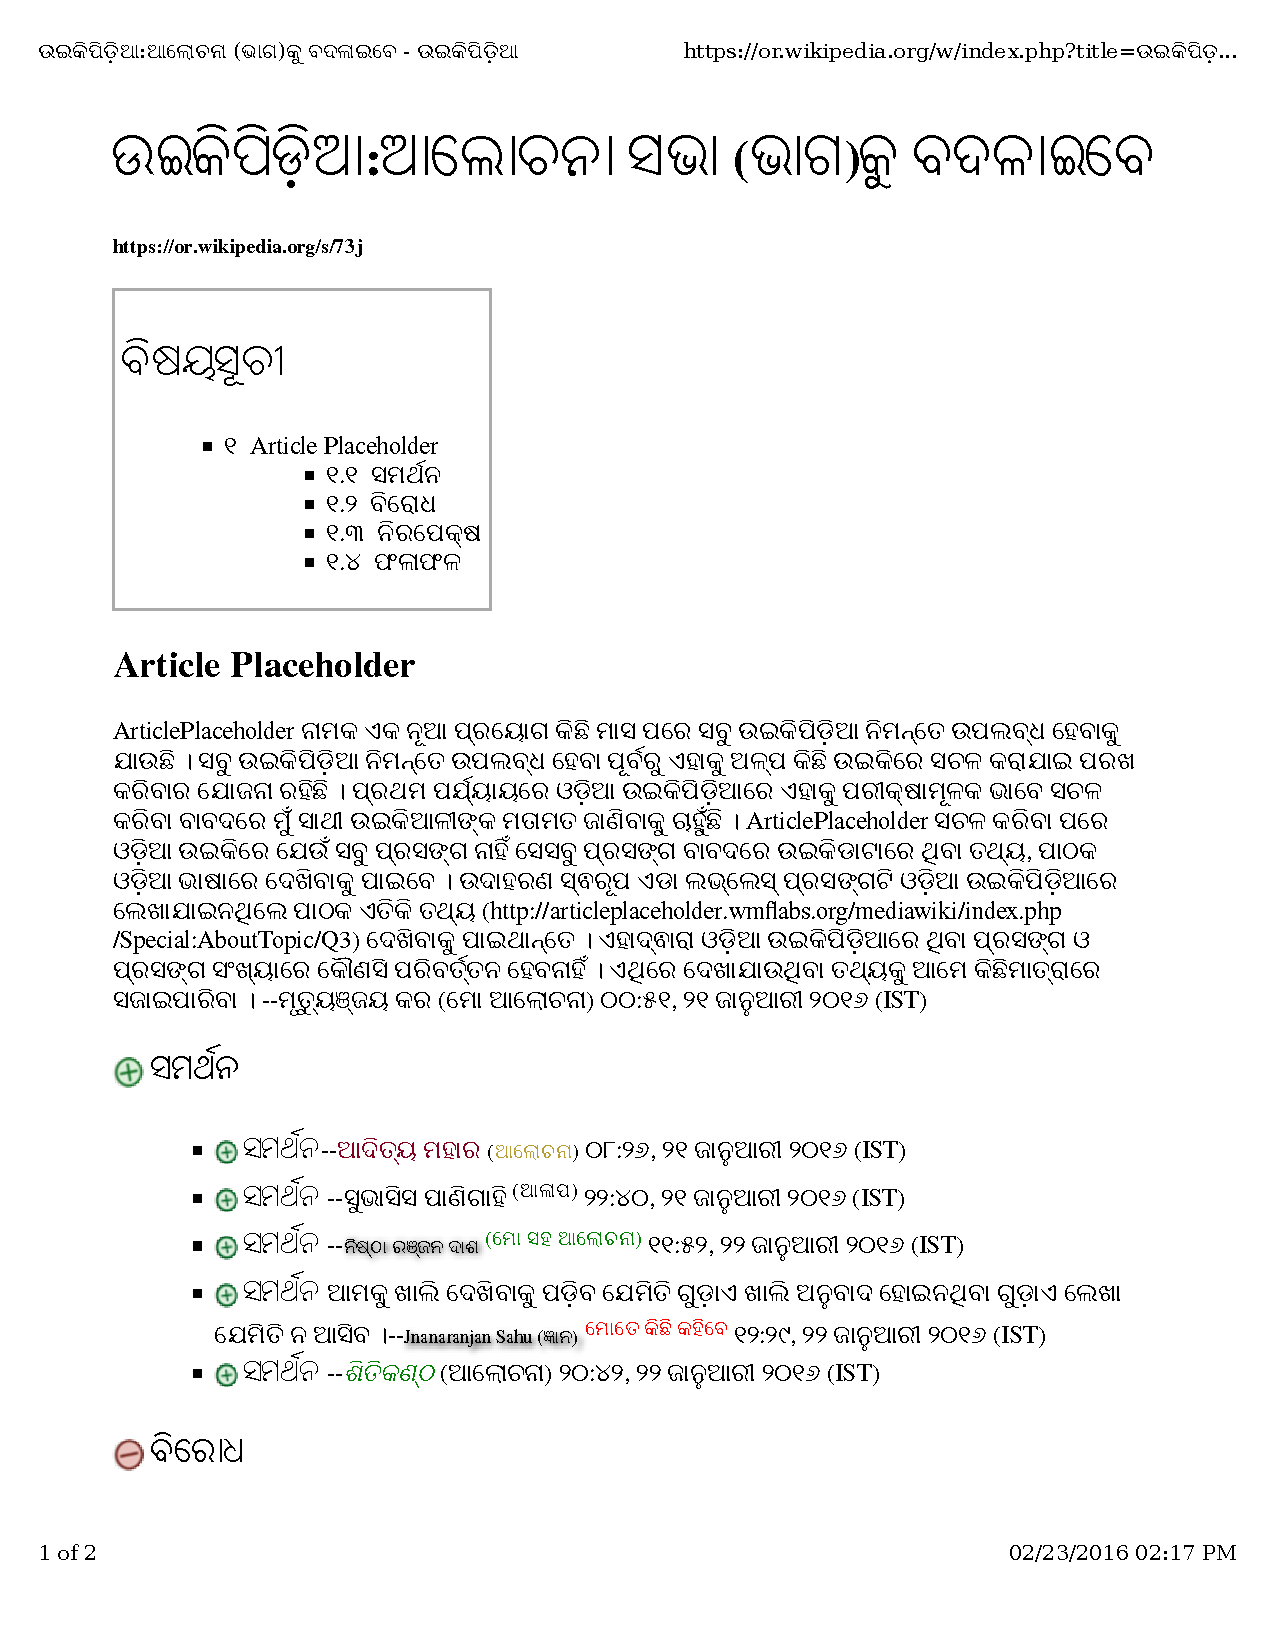
\includepdf[pages=1, scale=0.8, pagecommand={}, link, linkname=odwikipdf]{appendix/odwiki-discussion}
\includepdf[pages=2, scale=0.8, pagecommand={\footnotetext[1]{\cite{wiki:36}}}, link, linkname=odwikipdf]{appendix/odwiki-discussion}

%\hyperlink{odwikipdf.1}{odwikipages}

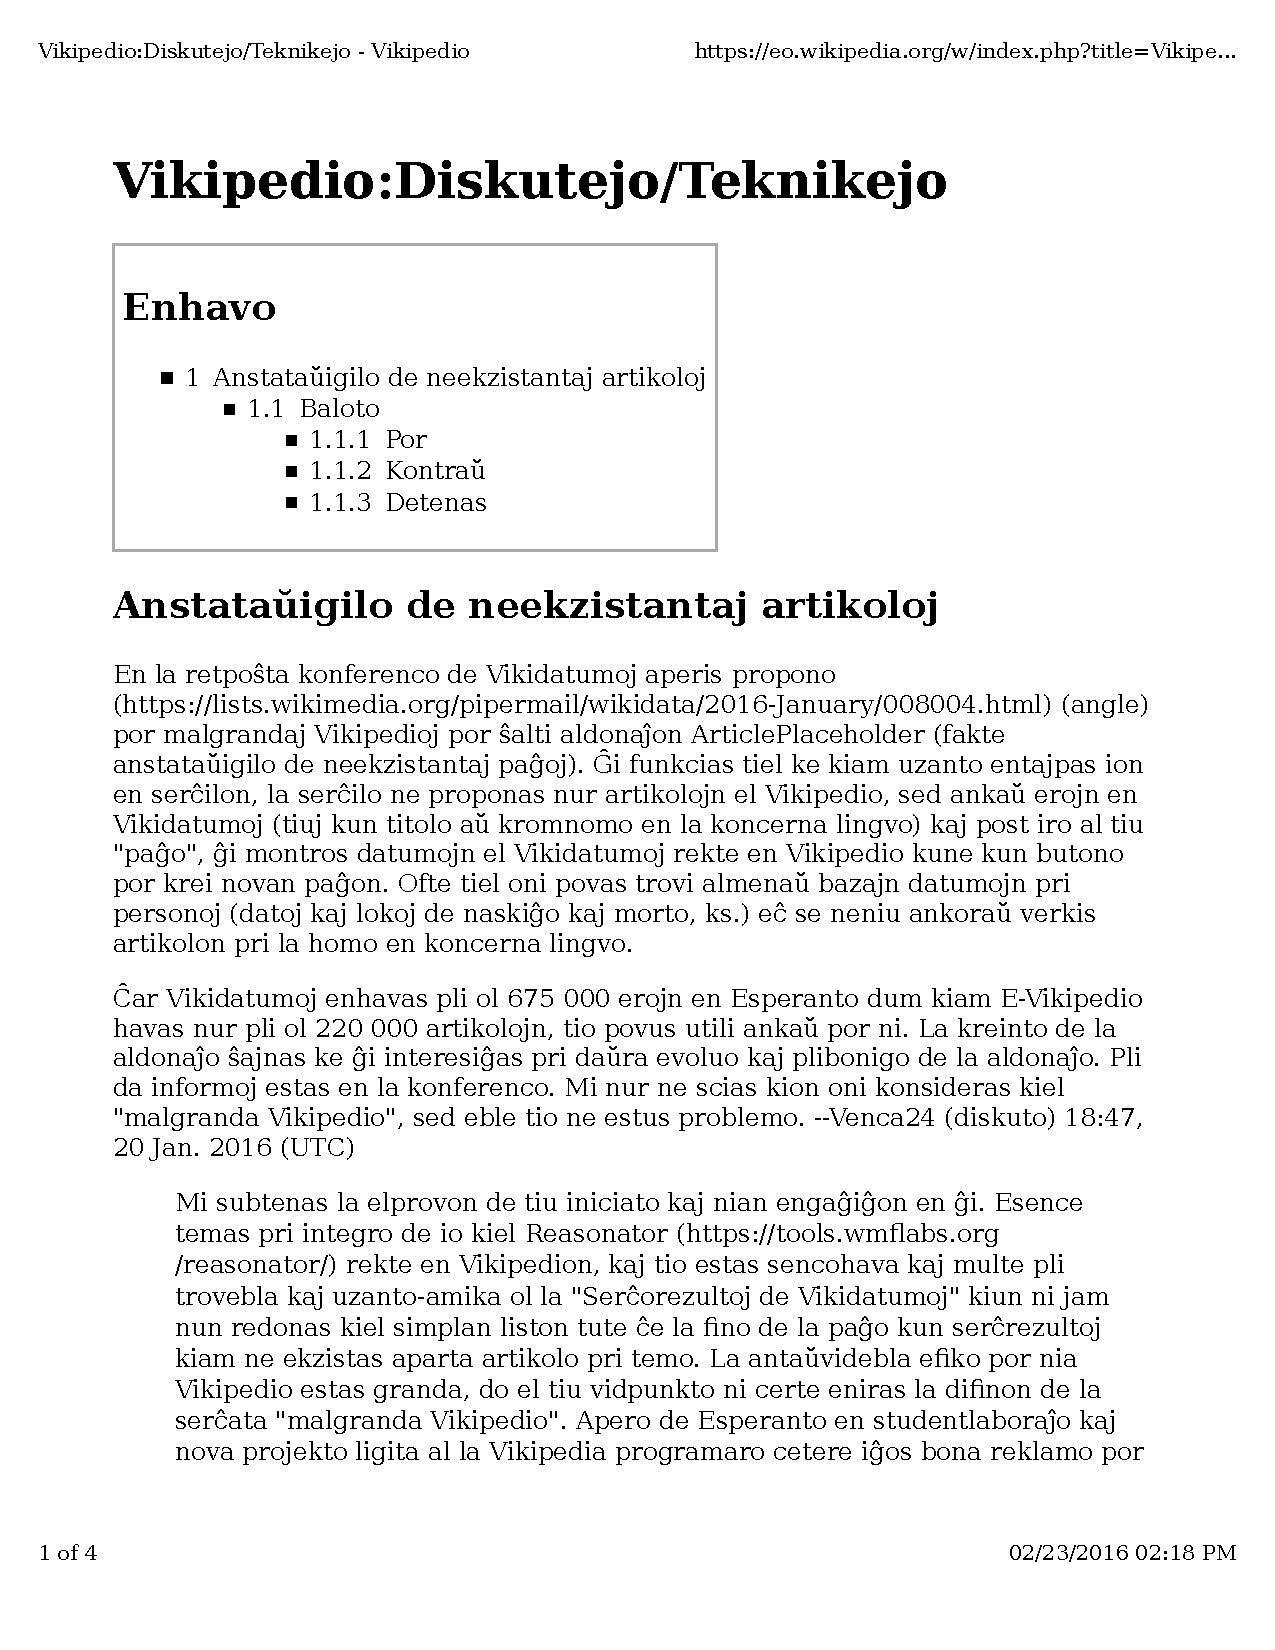
\includepdf[pages=1-3, scale=0.8, pagecommand={}, link, linkname=eowikipdf]{appendix/eowiki-discussion}
\includepdf[pages=4, scale=0.8, pagecommand={\footnotetext[1]{\cite{wiki:35}}}, link, linkname=eswikipdf]{appendix/eowiki-discussion}

